% =====================================================================
%  CUERPO DEL MANUAL DE ALMACÉN - PharmaWeigh
% =====================================================================

\seccion{1. Acceso al sistema}

\tablaAcceso

\vspace{8pt}

Para ingresar al sistema:
\begin{enumerate}
    \item Abre tu navegador web (Chrome recomendado).
    \item Ve a la dirección \cd{https://pharma-formweigh.vercel.app}.
    \item Ingresa tu \campo{email} y tu \campo{contraseña}.
    \item Haz clic en \boton{Ingresar}.
\end{enumerate}

\begin{center}
\fbox{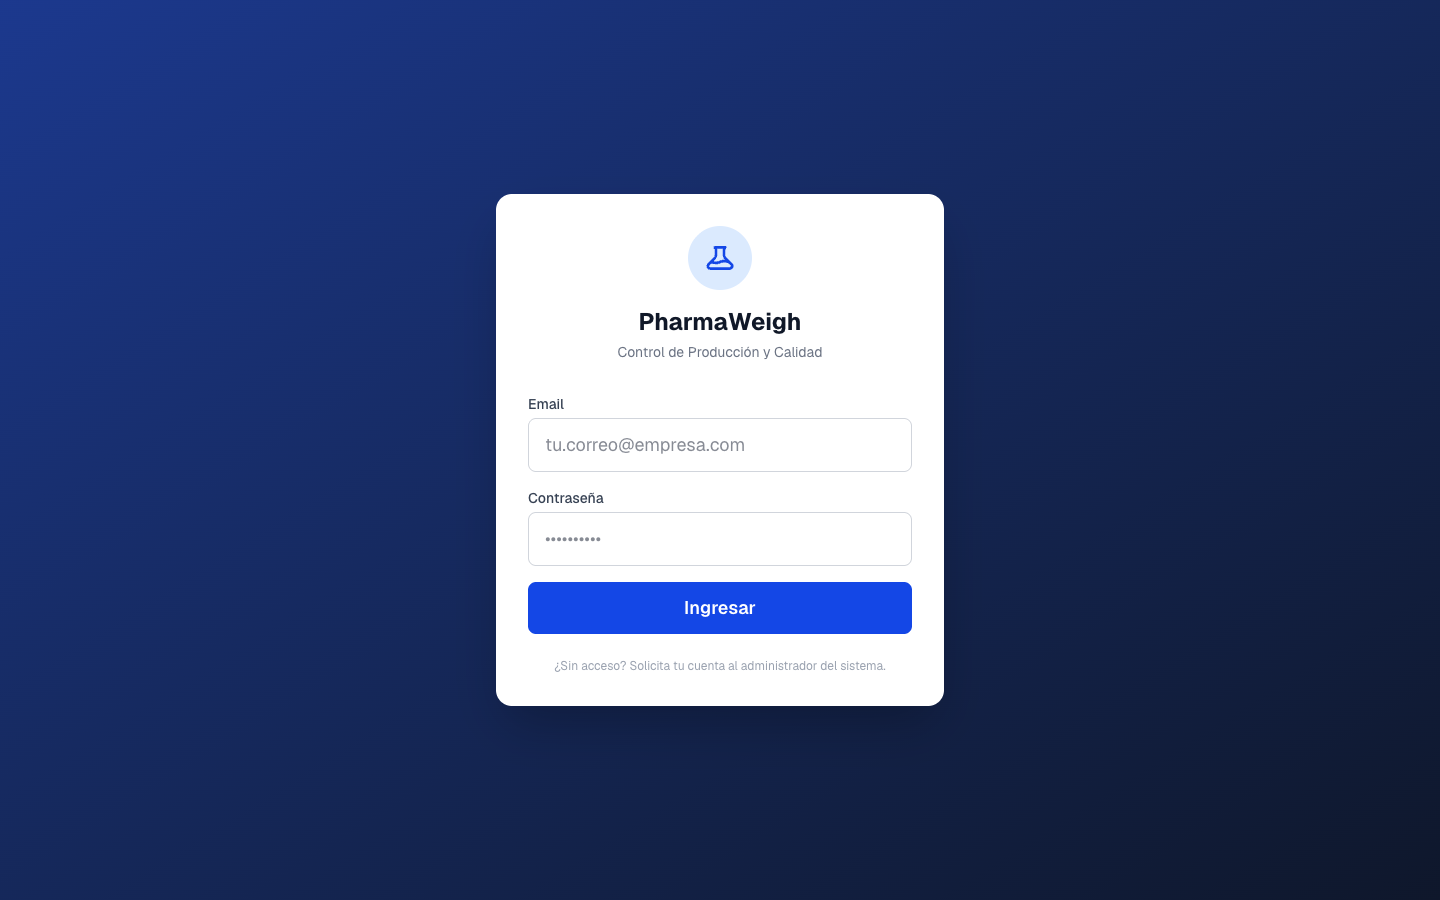
\includegraphics[width=0.85\linewidth]{capturas/01_login.png}}\\[3pt]
{\footnotesize\color{gristexto}Pantalla de inicio de sesión. Ingresa tu email y contraseña.}
\end{center}

Como \textbf{Almacenista}, tu función principal es recibir materias primas,
registrarlas en el sistema y mantener el inventario actualizado.

\begin{cajaNota}
\textbf{Tu menú lateral muestra:} Dashboard, Inventario, Códigos de Barras.
No tienes acceso a Recetas, Órdenes, Dispensado, Auditoría ni Usuarios.
\end{cajaNota}

% =====================================================================
\seccion{2. Tu rol en el proceso de producción}

Tú eres el \textbf{punto de entrada} de todas las materias primas al sistema:

\vspace{6pt}
\begin{center}
\begin{tikzpicture}[
    node distance=0.3cm and 1.2cm,
    every node/.style={font=\footnotesize},
    paso/.style={draw=pharmablue, fill=pharmablue!8, rounded corners=6pt,
        minimum width=2.6cm, minimum height=1cm, align=center, text width=2.4cm},
    tuyo/.style={draw=pharmagreen!80!black, fill=pharmagreen!15, rounded corners=6pt,
        minimum width=2.6cm, minimum height=1cm, align=center, text width=2.4cm,
        line width=1.5pt},
    flecha/.style={-{Stealth[length=5pt]}, thick, color=gristexto}
]
\node[tuyo] (recibir) {\textbf{1. ALMACÉN}\\Recibir materia\\prima};
\node[tuyo, right=of recibir] (registrar) {\textbf{2. ALMACÉN}\\Registrar lote\\en sistema};
\node[paso, right=of registrar] (calidad) {3. CALIDAD\\Aprobar lote};
\node[paso, below=1cm of recibir] (super) {4. SUPERVISOR\\Crear orden};
\node[paso, right=of super] (oper) {5. OPERARIO\\Dispensar};
\draw[flecha] (recibir) -- (registrar);
\draw[flecha] (registrar) -- (calidad);
\draw[flecha] (calidad) |- (super);
\draw[flecha] (super) -- (oper);
\end{tikzpicture}
\end{center}
\vspace{6pt}

Sin tu registro, el material \textbf{no existe} para el sistema y no puede
usarse en producción.

% =====================================================================
\newpage
\seccion{3. Dashboard}

\begin{center}
\fbox{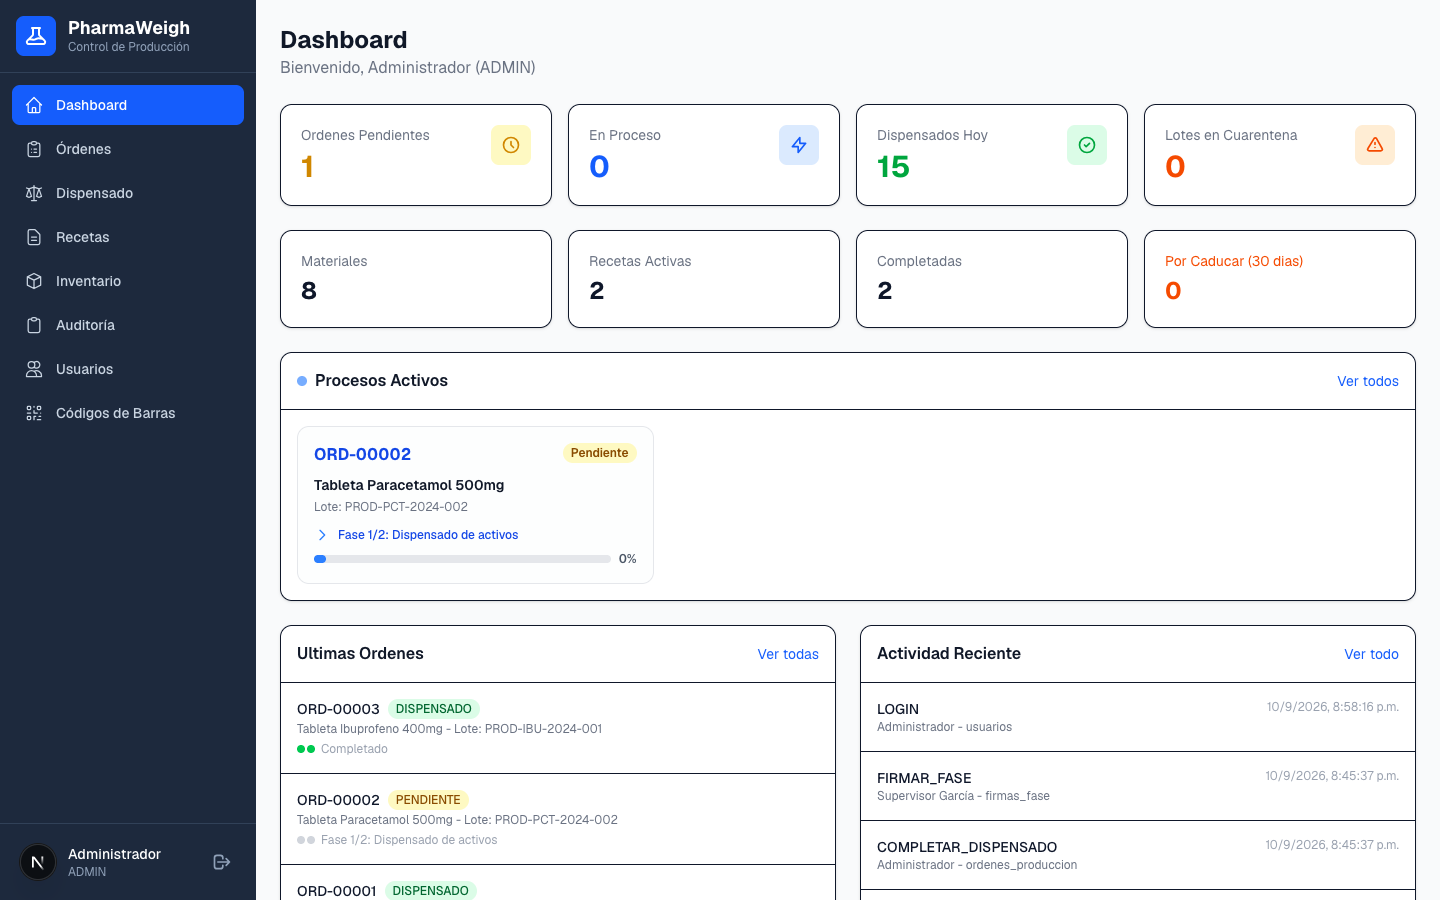
\includegraphics[width=0.92\linewidth]{capturas/03_dashboard.png}}\\[3pt]
{\footnotesize\color{gristexto}Dashboard principal con indicadores de producción.}
\end{center}

Como Almacenista, los indicadores clave son:
\begin{itemize}
    \item \textbf{Materiales:} total de materias primas en el sistema.
    \item \textbf{Lotes en Cuarentena:} lotes que registraste y esperan aprobación de Calidad.
    \item \textbf{Por Caducar (30 días):} lotes próximos a vencer --- coordina su uso prioritario.
\end{itemize}

% =====================================================================
\seccion{4. Equipo de trabajo}

\subseccion{4.1 Pistola láser (lector de código de barras)}

Tu herramienta principal es la \textbf{pistola láser} de código de barras.
La usas para identificar materiales rápidamente durante la recepción.

\begin{center}
\begin{tikzpicture}[
    every node/.style={font=\small}
]
% Pistola
\draw[fill=gray!15, draw=gray, rounded corners=3pt, line width=1pt]
    (0,0.5) -- (1.5,0.5) -- (2,1) -- (2,2.5) -- (1.5,3) -- (0,3) -- cycle;
\draw[fill=red!30, draw=red!60] (2,1.7) -- (3.5,1.2) -- (3.5,1.5) -- (2,2) -- cycle;
\node[font=\footnotesize\color{gristexto}] at (1,0) {Pistola láser USB};
\node[font=\tiny\color{red}] at (3.8,1.35) {Láser};

% Flecha
\draw[-{Stealth[length=6pt]}, thick, color=pharmablue] (4.2,1.5) -- (5.5,1.5);

% Etiqueta del material
\draw[fill=white, draw=gray, rounded corners=2pt]
    (5.8,0.3) rectangle (9.2,2.7);
\foreach \x in {6.1,6.3,6.4,6.7,6.8,7.1,7.2,7.4,7.7,7.8,8.0,8.2,8.4,8.6,8.8} {
    \draw[line width=1.2pt] (\x,0.8) -- (\x,2.2);
}
\node[font=\ttfamily\footnotesize] at (7.5,0.5) {MAT-PAR-001};
\end{tikzpicture}
\end{center}

La pistola funciona como un \textbf{teclado USB}:
\begin{itemize}
    \item Se conecta por USB a la computadora. No requiere drivers.
    \item Al escanear, envía los caracteres del código seguidos de \textbf{Enter}.
    \item El sistema identifica automáticamente el material por su código.
    \item Si la pistola no está disponible, puedes escribir el código manualmente.
\end{itemize}

\begin{cajaTip}[Tip]
Mantén la pistola siempre cargada (si es inalámbrica) o conectada (si es con cable).
Apunta el láser al \textbf{centro} del código de barras para una lectura rápida.
\end{cajaTip}

\subseccion{4.2 Báscula para recepción (ingreso manual)}

Al recibir material, necesitas pesar lo que llega. La báscula \textbf{no está
conectada} al sistema --- tú lees el peso en la báscula e ingresas la cantidad
manualmente en PharmaWeigh.

\begin{center}
\begin{tikzpicture}[
    every node/.style={font=\small}
]
\draw[fill=gray!10, draw=gray, rounded corners=4pt, line width=1pt]
    (0,0) rectangle (5,3);
\draw[fill=white, draw=gray!60, rounded corners=2pt]
    (0.5,1.5) rectangle (4.5,2.7);
\node[font=\Large\bfseries\color{pharmaazul}] at (2.5,2.1) {25.00 kg};
\node[font=\footnotesize\color{gristexto}] at (2.5,0.7) {Báscula de recepción};

\draw[-{Stealth[length=6pt]}, thick, color=pharmablue] (5.3,1.5) -- (7,1.5)
    node[midway, above, font=\footnotesize\color{gristexto}] {Tú lees y};
\node[draw=pharmablue, fill=pharmablue!5, rounded corners=4pt,
    minimum width=2.5cm, minimum height=1.5cm, align=center]
    at (8.5,1.5) {Ingresas la\\cantidad en\\PharmaWeigh};
\end{tikzpicture}
\end{center}

% =====================================================================
\newpage
\seccion{5. Recepción de materia prima}

Este es tu proceso principal. Cada vez que llega material a la planta,
debes registrarlo en el sistema.

\subseccion{5.1 Proceso paso a paso}

\begin{enumerate}
    \item Ve a \menu{Inventario} $\rightarrow$ pestaña \menu{Recepción}.

    \item \textbf{Escanea el código de barras del material} con la pistola láser.
        \begin{itemize}
            \item Apunta la pistola al código impreso en la etiqueta del material.
            \item El campo se llena automáticamente.
            \item El sistema muestra el nombre del material encontrado.
        \end{itemize}

    \item Si el material se identifica correctamente, llena los datos del lote:
        \begin{itemize}
            \item \campo{Número de Lote}: el identificador que trae el proveedor
                  (ej: \codigo{LOT-PAR-2024-003}).
            \item \campo{Cantidad}: pesa el material en la báscula e ingresa
                  la cantidad (ej: 25 kg).
            \item \campo{Proveedor}: nombre del proveedor.
            \item \campo{Fecha de Caducidad}: fecha de vencimiento del lote.
            \item \campo{Certificado de Análisis}: número de referencia del
                  certificado del proveedor (opcional).
        \end{itemize}

    \item Haz clic en \boton{Registrar Lote (Cuarentena)}.

    \item El lote se crea automáticamente en estado \cuarentena.
          \textbf{Calidad} lo revisará y aprobará después.
\end{enumerate}

\begin{center}
\fbox{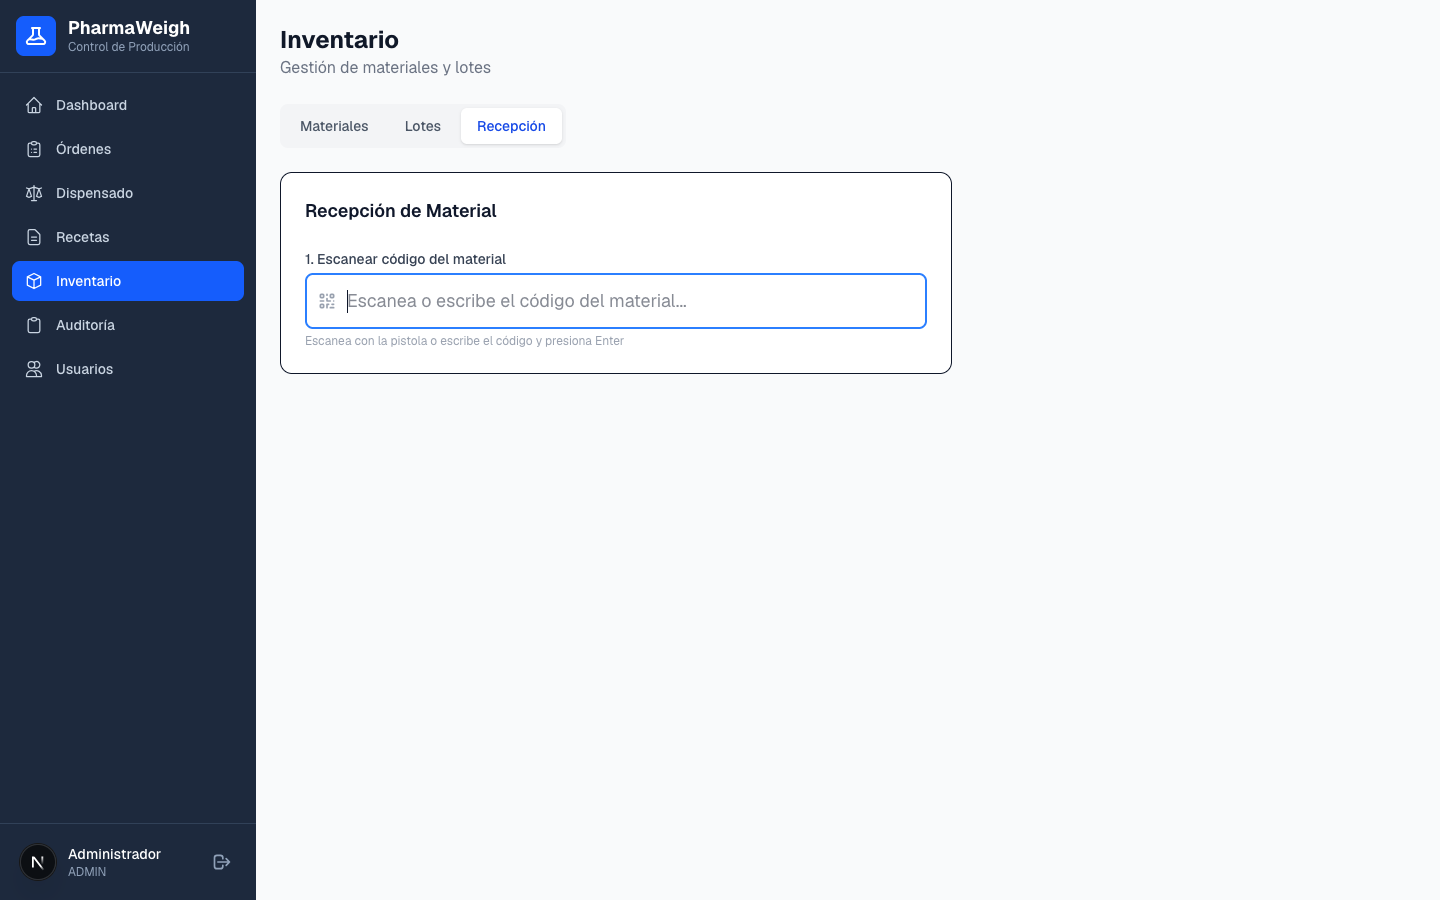
\includegraphics[width=0.92\linewidth]{capturas/16_inventario_recepcion.png}}\\[3pt]
{\footnotesize\color{gristexto}Pantalla de recepción: escanea el material con la pistola y llena los datos del lote.}
\end{center}

\begin{cajaOjo}
\textbf{Todo lote nuevo entra en CUARENTENA.} Esto significa que no puede usarse
en producción hasta que Calidad lo apruebe. Es una medida de seguridad del proceso
farmacéutico (BPM/GMP).
\end{cajaOjo}

% =====================================================================
\newpage
\seccion{6. Gestión de materiales}

\subseccion{6.1 Dar de alta un material nuevo}

Si llega un material que no existe en el sistema, tú puedes crearlo:

\begin{enumerate}
    \item Ve a \menu{Inventario} $\rightarrow$ pestaña \menu{Materiales}.
    \item Haz clic en \boton{+ Nuevo Material}.
    \item Llena los campos:
        \begin{itemize}
            \item \campo{Código}: el código de barras del material (ej: \codigo{MAT-PAR-001}).
                  Este es el código que escaneará la pistola.
            \item \campo{Nombre}: nombre completo del material.
            \item \campo{Unidad}: kg, g, L, mL, mg o unidad.
            \item \campo{Stock Mínimo}: umbral de alerta. Si el stock baja de este
                  valor, el material se resalta en \textbf{rojo} en el inventario.
        \end{itemize}
    \item Haz clic en \boton{Crear Material}.
\end{enumerate}

\begin{center}
\fbox{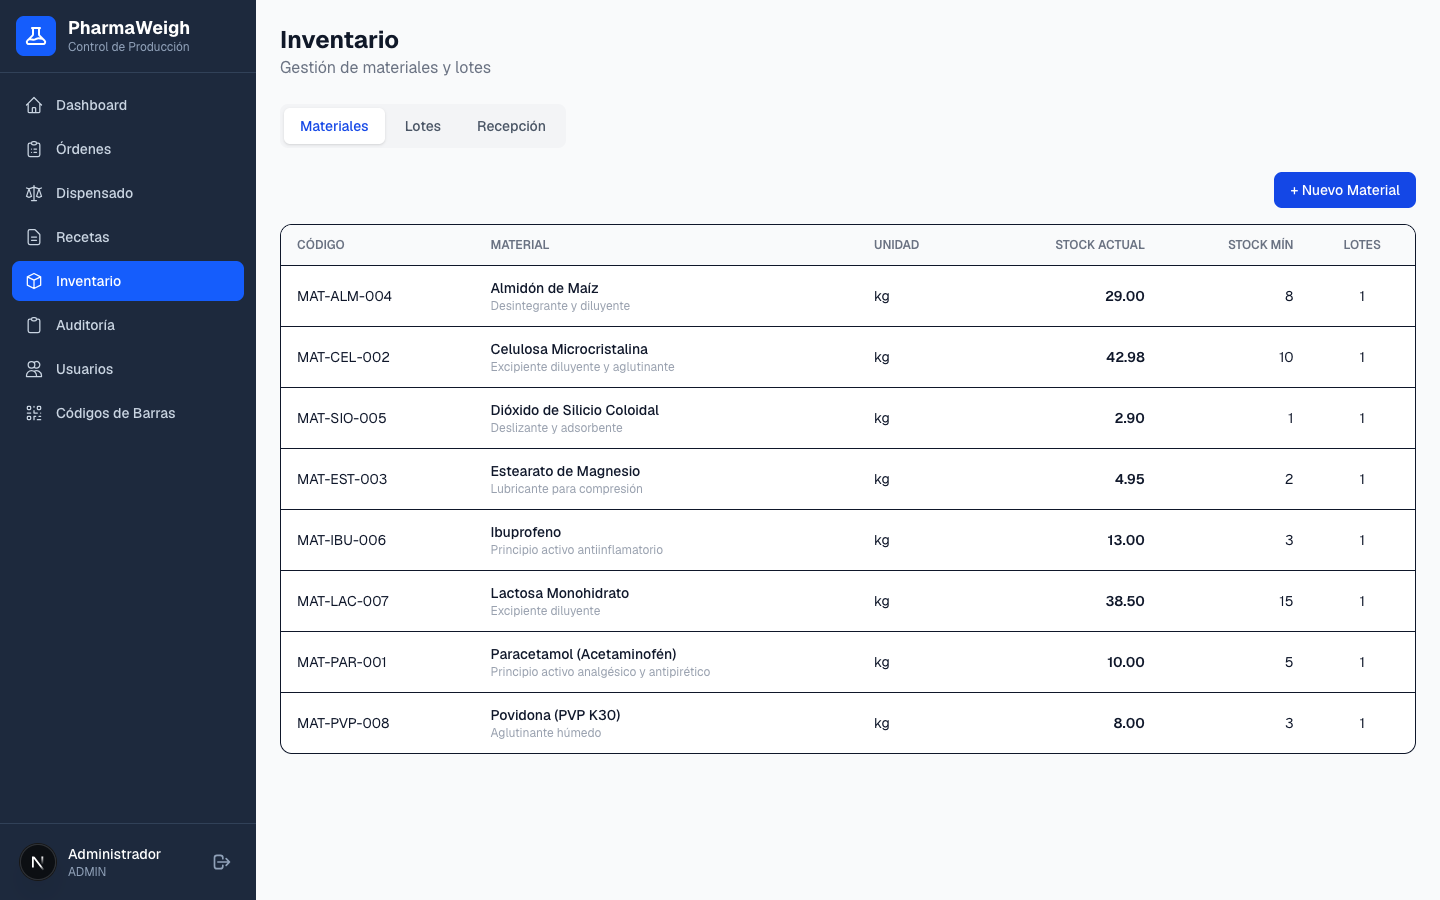
\includegraphics[width=0.92\linewidth]{capturas/14_inventario_materiales.png}}\\[3pt]
{\footnotesize\color{gristexto}Lista de materiales con código, stock actual, stock mínimo y lotes activos.
Los materiales con stock bajo se resaltan en rojo.}
\end{center}

\begin{cajaNota}
El \campo{Código} debe coincidir exactamente con el código impreso en las etiquetas
del material para que la pistola láser lo identifique correctamente.
\end{cajaNota}

\subseccion{6.2 Cambiar estado de lotes}

Como almacenista, puedes cambiar el estado de los lotes para reflejar
movimientos físicos:

\begin{itemize}
    \item Poner un lote en \cuarentena{} si detectas un problema físico.
    \item Marcar un lote como \agotado{} si se consumió completamente fuera del sistema.
\end{itemize}

\begin{cajaOjo}
La \textbf{aprobación definitiva} de lotes corresponde a \textbf{Calidad}.
Tú puedes mover estados para reflejar la realidad física del almacén,
pero el dictamen de calidad lo emite el área de QA.
\end{cajaOjo}

% =====================================================================
\newpage
\seccion{7. Consultar el inventario}

\subseccion{7.1 Pestaña Materiales}

Muestra todos los materiales registrados con su stock actual:

\begin{center}
\begin{tabularx}{\linewidth}{@{}l >{\raggedright\arraybackslash}X@{}}
\toprule
\textbf{Columna} & \textbf{Descripción} \\
\midrule
Código        & Código de barras del material \\
Nombre        & Nombre completo \\
Stock Actual  & Suma de todos los lotes aprobados \\
Stock Mínimo  & Umbral de alerta (rojo si el actual es menor) \\
Lotes Activos & Número de lotes con estado APROBADO o CUARENTENA \\
\bottomrule
\end{tabularx}
\end{center}

\subseccion{7.2 Pestaña Lotes}

\begin{center}
\fbox{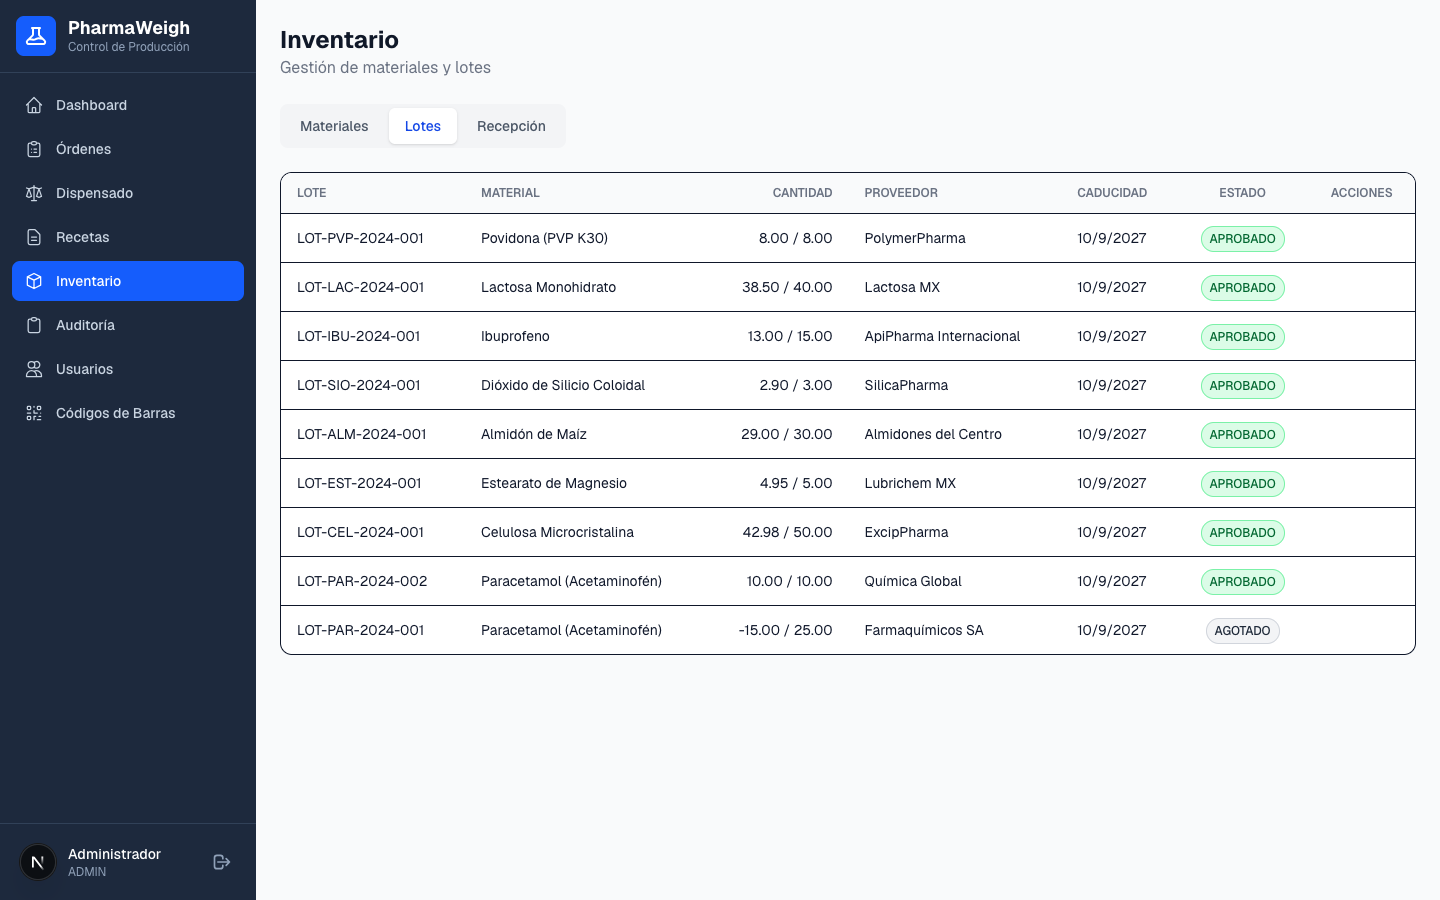
\includegraphics[width=0.92\linewidth]{capturas/15_inventario_lotes.png}}\\[3pt]
{\footnotesize\color{gristexto}Lista de lotes con estado, cantidad, proveedor y fecha de caducidad.}
\end{center}

Verifica regularmente:
\begin{itemize}
    \item \textbf{Lotes en cuarentena:} recuerda a Calidad que los apruebe.
    \item \textbf{Lotes próximos a caducar:} coordina con el supervisor para
          usarlos primero (FEFO: First Expired, First Out).
    \item \textbf{Stock bajo:} solicita reabastecimiento al área de compras.
\end{itemize}

% =====================================================================
\newpage
\seccion{8. Códigos de barras}

Desde \menu{Códigos de Barras} puedes ver e imprimir los códigos de todos
los lotes, materiales y badges del sistema.

\subseccion{8.1 Pestañas disponibles}

\begin{center}
\begin{tabularx}{\linewidth}{@{}l >{\raggedright\arraybackslash}X@{}}
\toprule
\textbf{Pestaña} & \textbf{Contenido} \\
\midrule
Lotes      & Códigos de barras de cada lote de materia prima \\
Materiales & Códigos de barras de cada material registrado \\
Badges     & Códigos de los gafetes de identificación de usuarios \\
\bottomrule
\end{tabularx}
\end{center}

\begin{cajaTip}[Tip]
Imprime los códigos de barras de los lotes nuevos y pégalos en los contenedores
físicos. Así el operario podrá escanearlos fácilmente durante el dispensado.
\end{cajaTip}

% =====================================================================
\seccion{9. Preguntas frecuentes}

\subseccion{¿Qué hago si el material no se encuentra al escanear?}
Significa que no está registrado en el sistema. Créalo primero en
\menu{Inventario} $\rightarrow$ \menu{Materiales} $\rightarrow$
\boton{+ Nuevo Material} y luego registra el lote.

\subseccion{¿Puedo modificar un lote ya registrado?}
Puedes cambiar su estado (cuarentena, aprobado, etc.) pero no la cantidad
original. Si hubo un error en la cantidad, registra un nuevo lote con los
datos correctos.

\subseccion{¿Qué pasa si la pistola no lee el código?}
Puedes \textbf{escribir el código manualmente} en el campo y presionar
\boton{Enter}. La pistola a veces no lee si el código está dañado,
sucio o tiene bajo contraste.

\subseccion{¿Quién puede crear materiales y registrar lotes?}
Solo usuarios con rol \textbf{ALMACEN}, \textbf{SUPERVISOR} o \textbf{ADMIN}.
Los demás roles pueden consultar el inventario pero no modificarlo.
